In the previous sections we discussed how neural networks are built up. Now we will give an example of how they can be trained and used to perform specific tasks. Specifically, we will look at how they can be trained on data sets in a process called \textbf{supervised learning}. For this we fix the architecture of our neural network, which includes the organisation of neurons, the input and output handling and the activation function. The things we can vary during training to make our network perform better are the parameters $\theta$.

\subsection{Datasets}
First we need to assume that we have a given dataset containing input-output pairs that represent the task we want the neural network to perform. The neural network is supposed to learn which output is supposed to be generated from an input by evaluating the given inputs and desired outputs. We will call those desired outputs "\textbf{targets}" to distinct them from the actual output of the neural network during training. A good example of this would be the MNIST database, which was first used in 1994 in \cite{firstMNISTpaper} as a modification of an earlier database, and has since become a popular entry-level classification task for machine learning. Examples of input data for this database are shown in \cref{fig:MNIST_examples}. 
\img{text/MachineLearningBasics/plots/mnist_plot.pdf}{14cm}{Displayed in this figure are 4 examples of input values for the MNIST dataset. This dataset represents handwritten digits from 0 to 9. Each input value consists of a 28 by 28 grid of grayscale pixel values.}{fig:MNIST_examples}
This dataset consists of various handwritten digits from 0 to 9 represented by a 28 by 28 grid of grayscale pixel values. The values of the pixels in these grids act as the 784 input values for the neural network, the targets should be shaped according to the output of the neural network. For example one might use a scalar output of the neural network that should be equal to the value of the digit drawn in the input pixel grid. In this case the targets are scalar values from 0 to 9 corresponding to their input pictures. Another way would be to use 10 output values together with the previously mentioned softmax function (see \cref{sec:NeuralNetworks}) to recieve the values as probabilities for the different numbers as output. We would then change our targets to vectors with 10 elements, where the entry corresponding to the handwritten digit in the input picture would be 1, every other value would be 0.\\
We will denote the data sets as mathematical sets of input-target pairs $\{(\mathbf{x}_i, \mathbf{y}_i)\}_{i=1}^N$, where $\mathbf{x}_i$ are the input values and $\mathbf{y}_i$ are the targets. Here we called the amount of training data $N$. The mathematical dimension of $\mathbf{x}_i$ and $\mathbf{y}_i$ can vary and are dependent on the network architecture, but we will assume that they are vectors of the real numbers $\mathbf{x}_i \in \mathbb{R}^a$ $\mathbf{y}_i \in \mathbb{R}^b$. Due to this property we also sometimes refer to them as "points". If our inputs values are organized in a different manner, for example the MNIST data being matrices of $\mathbb{R}^{28\times28}$ we can rearrange these numbers into a vector of $\mathbb{R}^{784}$ in any way we want. The only important thing is that we convert every data point into a vector in the same way.\\
Going further we will denote all the output values of the neural network for the input $\mathbf{x}_i$ by $f_\theta(\mathbf{x}_i)$. This means that we mathematically describe the whole behavior of the neural network as a function
\begin{equation}
	f: \mathbb{R}^a \times \mathbb{R}^p \rightarrow \mathbb{R}^b
\end{equation}
with $p$ being the amount of parameters in the network.

\subsection{Loss function}
Now we have defined what a neural network is and how the input data we want to train on is structured. In order to train our networks to behave according to our data set, we now need to introduce a way to measure how well our network is performing. Once we can evaluate the performance of our network, we can then introduce ways to optimize that performance.\\
This measure of the performance of a neural network is called the "\textbf{loss function}" $\mathscr{L}$. It is also sometimes referred to as the cost function in literature. For this study we will only consider loss functions of the form 
\begin{equation}
	\mathscr{L}\left( \{(\mathbf{x}_i, \mathbf{y}_i)\}_{i=1}^{N}, \theta \right) = \frac{1}{N} \sum_{i=1}^{N} \ell_\theta\left(\mathbf{x}_i,\mathbf{y}_i\right).
	\label{eq:Loss_longform}
\end{equation}
As a reminder, $\theta$ is a set containing the parameters of the neural network. This is the variable of the loss function that describes the neural network. How one calculates the output of the neural network using the inputs and $\theta$ has to be intrinsically defined as well. Sometimes it's more convenient to also denote this dependency, which would make the loss function
\begin{equation}\label{eq:Loss_longform_withFunctiondependency}
	\mathscr{L}\left( \{(f_\theta(\mathbf{x}_i), \mathbf{y}_i)\}_{i=1}^{N} \right) = \frac{1}{N} \sum_{i=1}^{N} \ell_\theta\left(f_\theta(\mathbf{x}_i),\mathbf{y}_i\right).
\end{equation}
How exactly the loss function should be defined cannot be generally stated. The only thing certain is that the value of the loss function should generally be smaller the closer the output of the neural network is to the corresponding targets.\\
In most of our cases we use loss functions with 
\begin{equation}
	\ell_\theta \left( \mathbf{x}_i,\mathbf{y}_i\right) = 
	d\left(f_\theta(\mathbf{x}_i), \mathbf{y}_i\right),
\end{equation}
where $d$ represents the distance between the output vector of the neural network and the target vector according to different metrics. One very simple example would be 
\begin{equation}
	\mathscr{L}\left( \{(\mathbf{x}_i, \mathbf{y}_i)\}_{i=1}^{N}, \theta \right) = \frac{1}{N} \sum_{i=1}^{N} \sum_{j=1}^{N} \left(f_\theta(\mathbf{x}_i)_j - y_{i,j}\right)^2,
\end{equation}
with $f_\theta(\mathbf{x}_i)_j$ and $y_{i,j}$ being the $j$-th component of the network output and target vectors. Further examples and more general loss functions can be seen in \cite{LossExamplePaper}.

\subsection{Optimization}\label{sec:NetworkOptimization}
To quickly recap, we have now defined what a neural network is and that we want a fixed network architecture during training whose parameters we can vary to optimize the performance. We also assume that we have a data set that we want our network to behave like and a loss function that measures how well the current setup of our network is performing. We will now talk about how we can change the parameters in an attempt to optimize performance, which is achieved by lowering the value of the loss function.\\
The simplest and most common algorithm to do this with is \textbf{Gradient Descent} (GD). Here, the rule for updating the parameters looks like 
\begin{equation}\label{eq:GD}
	\theta' = \theta - \eta \nabla_\theta \mathscr{L}\left[ \{(\mathbf{x}_i, \mathbf{y}_i)\}_{i=1}^{N}, \theta \right],
\end{equation}
where $\eta$ is a parameter of training called the "learning rate", which is a scalar value for GD but could also vary through training and even be a tensor for more advanced optimization methods.\\
The idea behind this is that the gradient with respect to $\theta$ points in the direction of the steepest ascent of the loss when the parameters are varied. If we subtract this gradient from the parameters we change the loss in the opposite direction, which is the direction of steepest descent. To visualize this, lets examine a single parameter that we will call $\theta_1$. The update rule for this single parameter can be obtained from writing out the previous \cref{eq:GD} in its full vectorial component form and then picking out the line of $\theta_1$. It reads
\begin{equation}
	\theta_1' = \theta - \eta \pAbl{}{\theta_1} \mathscr{L}\left[ \{(\mathbf{x}_i, \mathbf{y}_i)\}_{i=1}^{N}, \theta \right].
\end{equation}
To explain the concept of this algorithm more visually let's take a look at \cref{fig:gd_explanation_plot}. 
\begin{figure}
	\centering
	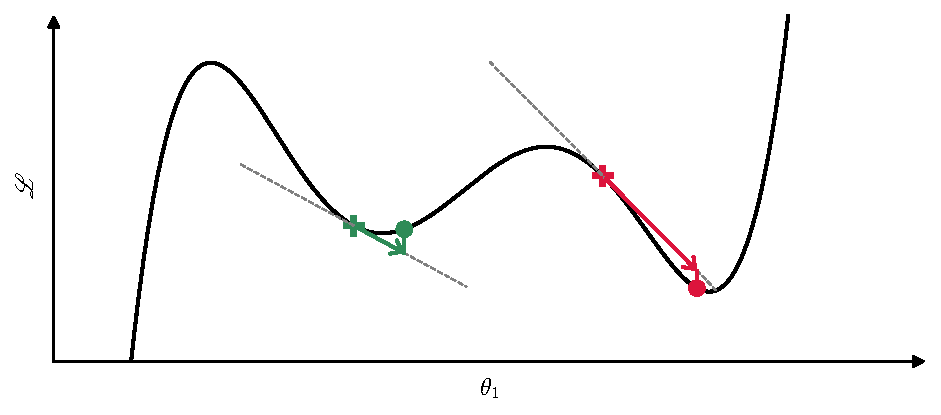
\includegraphics[width = 14cm]{text/MachineLearningBasics/plots/sgd_plot.pdf}
	\caption{This figure shows a visual explanation for the Gradient Descent algorithm. The dot markers show where a parameter that starts at the cross marker might end up if the algorithm is applied.}
	\label{fig:gd_explanation_plot}
\end{figure}
Here the cross markings symbolize the position of parameter $\theta_1$ before the update step. The algorithm then calculates the derivative of the loss $\pAbl{}{\theta_1} \mathscr{L}$, which is the slope of the tangent. Now, to change the parameter, the slope is multiplied with $-1$ times the learning rate $\eta$ and added to $\theta_1$, which is represented by the arrows. These arrows are adjusted in length so that the distance they cover in the direction of $\theta_1$ is $\eta$ times the derivative. They point in the direction of the tangent to show their dependence on the slope. One can see that the red arrow on the right covers more distance in the direction of $\theta_1$ than the green one on the left, which is a result of the corresponding slope being steeper. The circle markers then represent where the parameter values end up after the update step.\\
This visual example already illustrates some of the drawbacks of the GD algorithm. For example, the green starting parameter will end up in a local minimum that has a higher loss value than the local minimum that the red parameter value tends to. Also going further to the left would make the loss function smaller than both of these local minima. GD just tends to find the closest local minimum instead of a global one. Another drawback results from the step size being finitely big, which makes the green parameter hop over the local minimum. Both of these problems can't be solved by simply optimizing the learning rate $\eta$ in general.

\subsection{Other optimizers}
The GD calculates the gradient from the whole data set, although in most cases it is sufficient or even beneficial to compute the loss function and its gradient for a subset of the whole data set, which is usually called a batch or mini-batch. The extreme end of this would be to calculate the gradient and update the parameters for one data point each, which is then called \textbf{stochastic Gradient Descent}.
GD and the variations are very simple and fast to compute algorithms, but they can only find local minima and can quite easily hop over the actual minima. That's why other algorithms have been developed that try to solve or mitigate some of the problems of GD. For the training, which will be performed later in this thesis, the so-called ADAM optimizer was used. The intricacies of this optimization method are beyond the scope of this work. We refer the interested reader to \cite{adamPaper}, where the details of this algorithm are discussed. Another optimization algorithm that can be used to overcome some of the problems of GD is the Natural Gradient Descent, which will be mentioned in later sections.


